\chapter{Logistic Regression}
\label{ch:logistic_regression}

Logistic regression is one of the best-known classifiers. The model returns the probability of a class variable, based on input features. First, it computes probabilities with a one-versus-all approach, meaning that for a multiclass problem, it will take one target value and treat all the rest as "other", effectively transforming the problem to binary classification.

Second, it tries to find an optimal plane that separates instances with the target value from the rest. Then it uses logistic function to transform the distance to the plane into probabilities. The further away from the plane an instance will be, the higher the probability it belongs to the class on that side of the plane. The closer it is to the decision boundary (the plane), the more uncertain the prediction becomes (i.e. it gets close to 0.5).

\begin{marginfigure}
    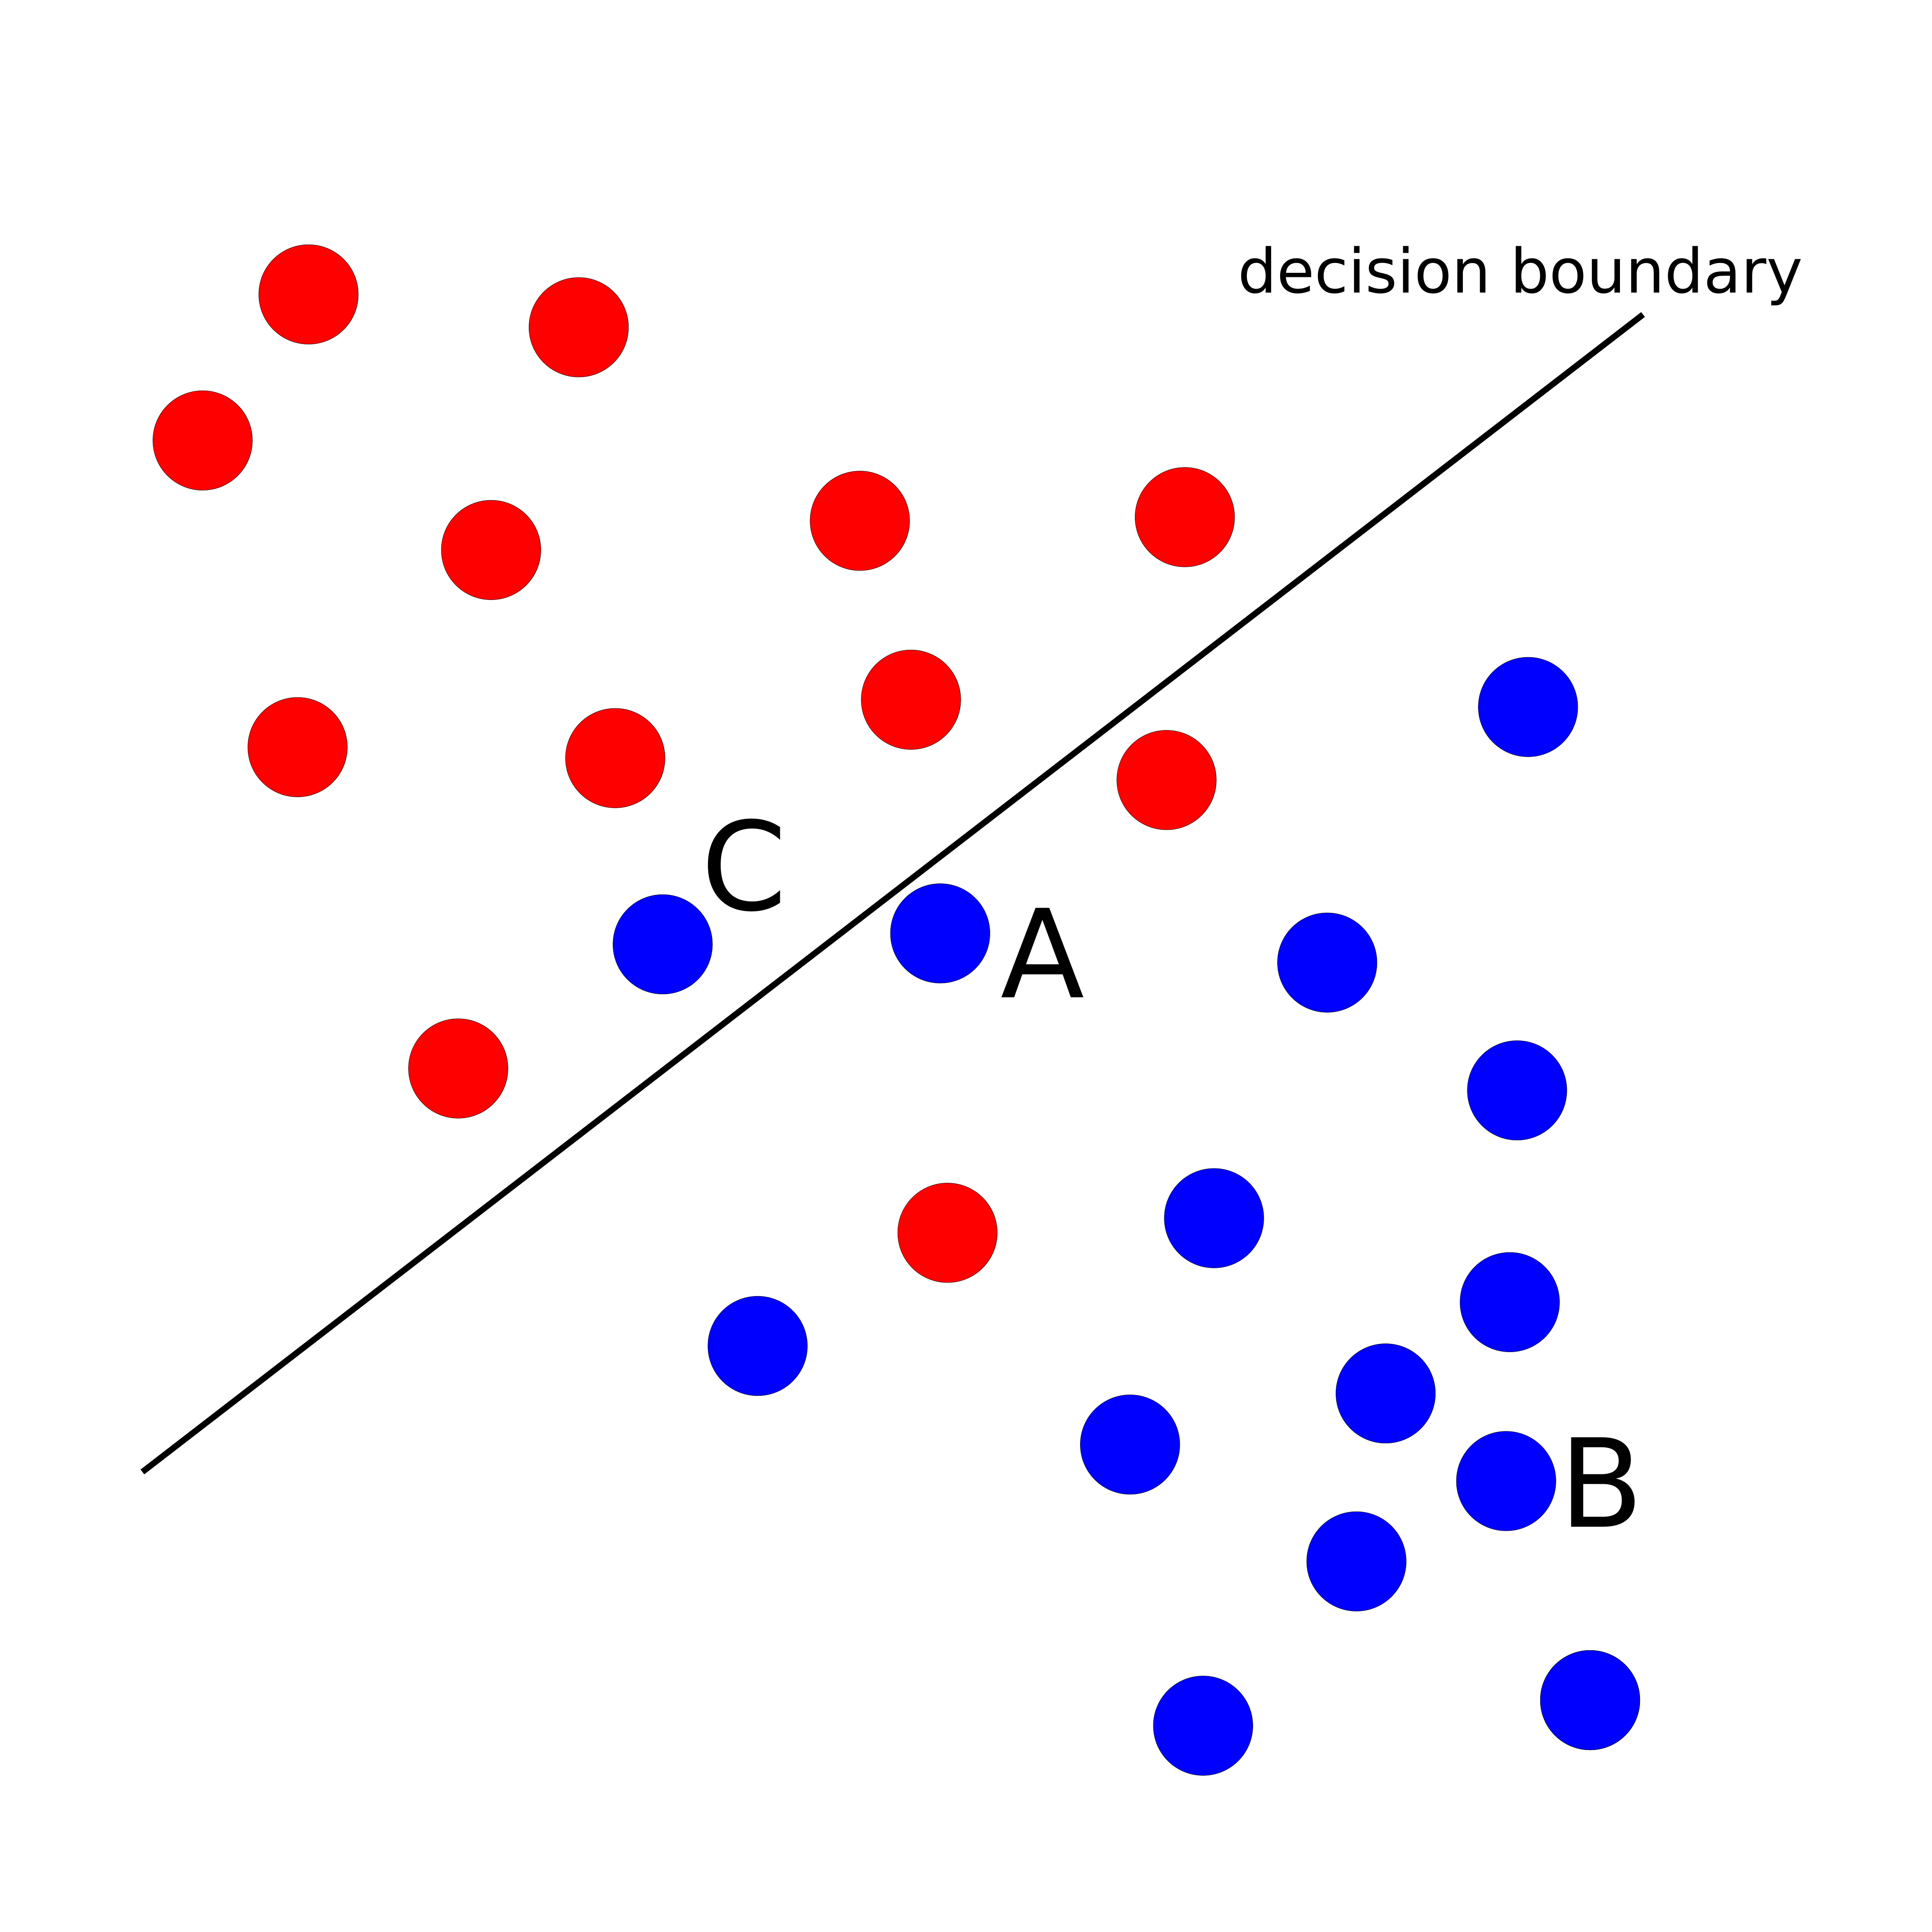
\includegraphics[width=60mm]{logistic-regression.png}%
    \caption{Can you guess what would the probability for belonging to the blue class be for A, B, and C?}
    \label{fig:logreg}
  \end{marginfigure}

Logistic regression tries to find such a plane that all points from one class are as far away from the boundary (in the correct direction) as possible.

\begin{marginfigure}
    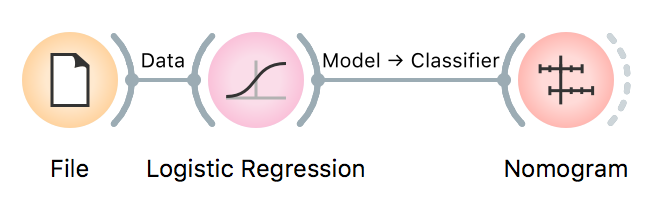
\includegraphics[width=60mm]{workflow.png}%
    \label{fig:workflow}
  \end{marginfigure}

A great thing about \widget{Logistic Regression} is that we can interpret it with a \widget{Nomogram}. Nomogram shows the importance of variables for the model. The higher the variable is in the list, the greater its importance. Also, the longer the line, the greater the importance. The line corresponds to the coefficient of the variable, which is then mapped to the probability. You can drag the blue point on the line left or right, decreasing or increasing the probability of the target class. This will show you how different values affect the outcome of the model.

\begin{figure}[h]
    \centering
    \vspace{-0.2cm}
    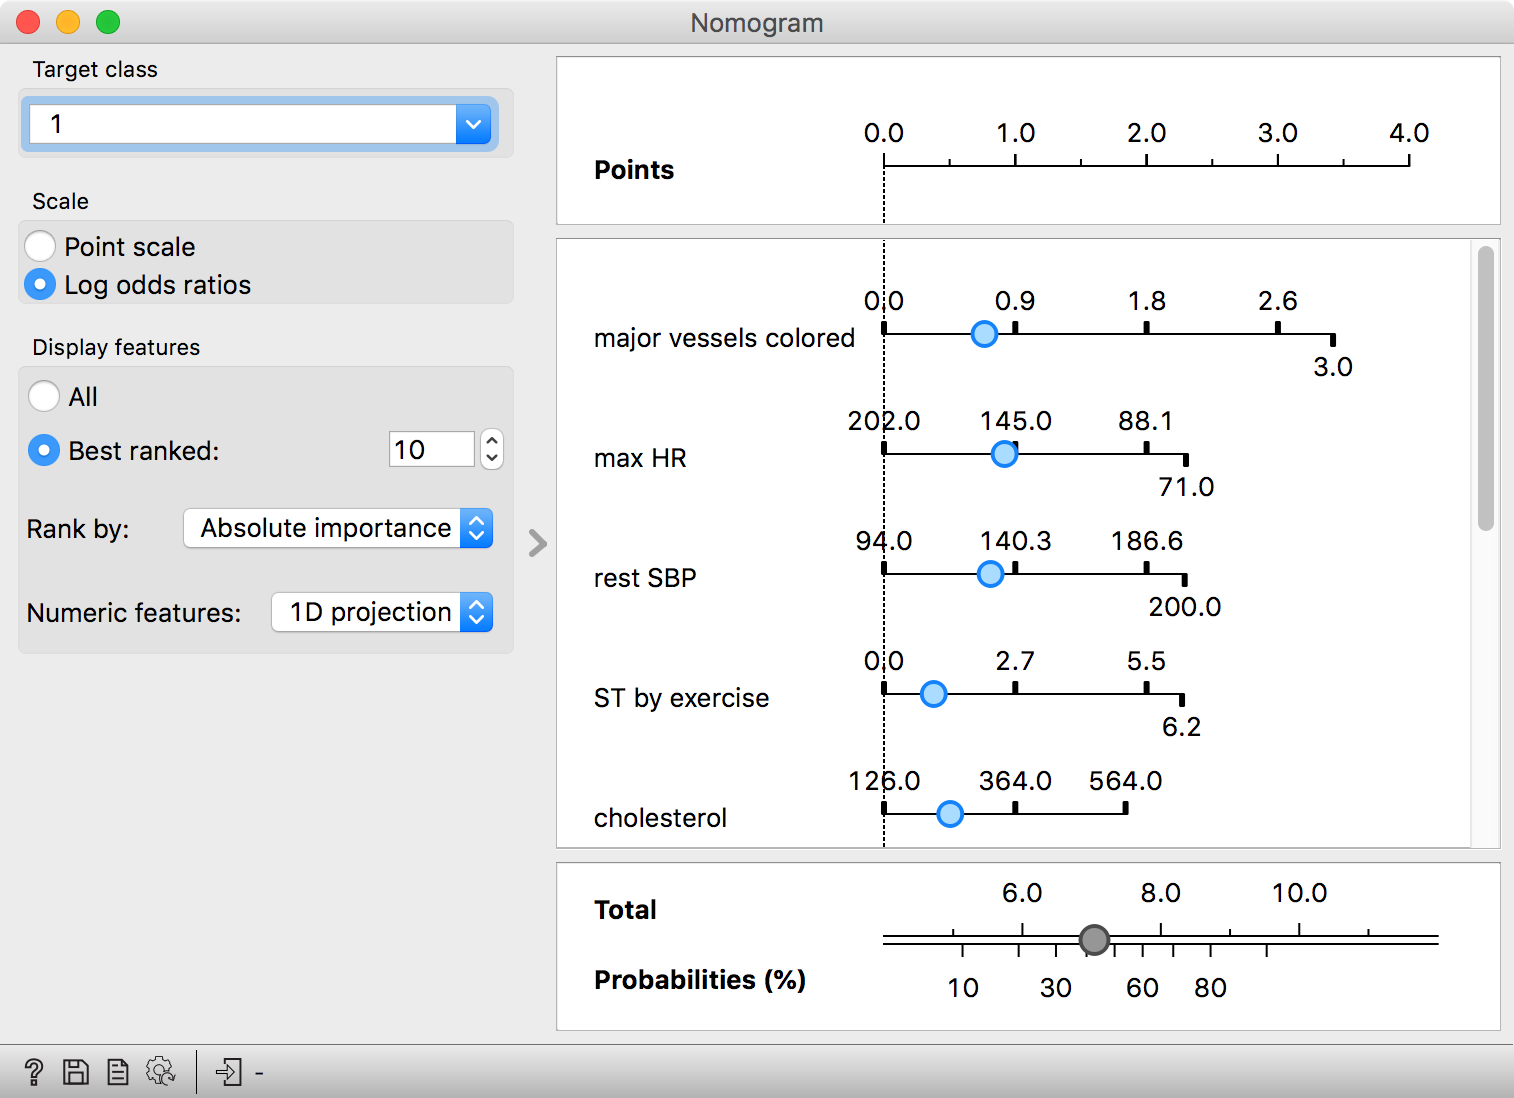
\includegraphics[scale=0.4]{nomogram.png}
\end{figure}

Another characteristic of logistic regression is that it observes all variables at once and takes the correlation into account. If some variables are correlated, their importance will be spread among them.

A not so great thing about logistic regression is that it operates with planes, meaning that the model won't work when the data cannot be separated in such a way. Can you think of such a data set?
